\documentclass[10pt, a4paper]{scrartcl}

\usepackage{vorschule}
\usepackage[
    typ=ab,
    fach=Informatik,
    lerngruppe={Q1-GK},
    nummer=PA001,
    module={Symbole,Lizenzen},
    seitenzahlen=keine,
    farbig,
    lizenz=cc-by-nc-sa-4,
]{schule}

\usepackage[
	kuerzel=Ngb,
	reihe={Objektorientierte Programmierung},
	version={2019-11-19},
]{ngbschule}

\author{J. Neugebauer}
\title{Tic-Tac-Toe}
\date{\Heute}

\setzeAufgabentemplate{ngbnormal}

%\usepackage{qrcode}

\begin{document}

\ReiheTitel

Implementieren sie das Spiel \enquote{Tic-Tac-Toe} in Java unter Verwendung von \emph{zweidimensionalen Arrays} als Datenstruktur.

\bigskip
\begin{minipage}{\textwidth-4cm}
\begin{quote}
\textbf{Tic-Tac-Toe}

Auf einem quadratischen, 3×3 Felder großen Spielfeld setzen die beiden Spieler abwechselnd ihr Zeichen (ein Spieler Kreuze, der andere Kreise) in ein freies Feld. Der Spieler, der als Erster drei Zeichen in eine Zeile, Spalte oder Diagonale setzen kann, gewinnt. Wenn allerdings beide Spieler optimal spielen, kann keiner gewinnen, und es kommt zu einem Unentschieden. Das heißt, alle neun Felder sind gefüllt, ohne dass ein Spieler die erforderlichen Zeichen in einer Reihe, Spalte oder Diagonalen setzen konnte.

\begin{flushright}\footnotesize
Quelle: \href{https://de.wikipedia.org/wiki/Tic-Tac-Toe}{https://de.wikipedia.org/wiki/Tic-Tac-Toe}
\end{flushright}
\end{quote}
\end{minipage}\hfill\begin{minipage}{4cm}
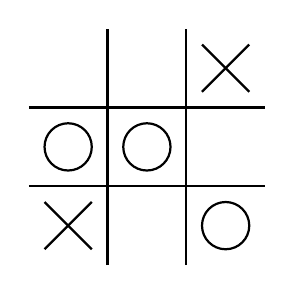
\begin{tikzpicture}
	\draw[thick] (1,0) -- +(0,3);
	\draw[thick] (2,0) -- +(0,3);
	\draw[thick] (0,1) -- +(3,0);
	\draw[thick] (0,2) -- +(3,0);
	
	\draw[thick] (.2,.2) -- (.8,.8);
	\draw[thick] (.2,.8) -- (.8,.2);
	\draw[thick] (2.2,2.2) -- (2.8,2.8);
	\draw[thick] (2.2,2.8) -- (2.8,2.2);
	
	\draw[thick] (.5,1.5) circle (.3);
	\draw[thick] (1.5,1.5) circle (.3);
	\draw[thick] (2.5,.5) circle (.3);
\end{tikzpicture}
\end{minipage}

\bigskip
Im Programm sollen zwei Spieler im Wechsel ziehen können, bis einer gewonnen hat. Die Wahl des Spielfeldes erfolgt jeweils durch die Eingabe der Feldkoordinaten (siehe Abbildung) auf der Kommandozeile.
\begin{center}
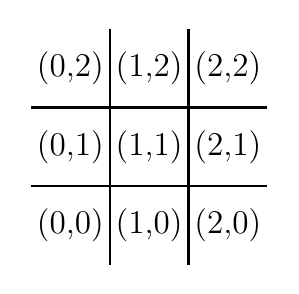
\begin{tikzpicture}
	\draw[thick] (1,0) -- +(0,3);
	\draw[thick] (2,0) -- +(0,3);
	\draw[thick] (0,1) -- +(3,0);
	\draw[thick] (0,2) -- +(3,0);
	
	\node at (.5,.5) {\large (0,0)};
	\node at (1.5,.5) {\large (1,0)};
	\node at (2.5,.5) {\large (2,0)};
	\node at (.5,1.5) {\large (0,1)};
	\node at (1.5,1.5) {\large (1,1)};
	\node at (2.5,1.5) {\large (2,1)};
	\node at (.5,2.5) {\large (0,2)};
	\node at (1.5,2.5) {\large (1,2)};
	\node at (2.5,2.5) {\large (2,2)};
\end{tikzpicture}
\end{center}

Die Ausgabe des Spielfeldes kann als Text auf der Kommandozeile vorgenommen werden.

\bigskip
\textbf{Tipps:}
\begin{itemize}
	\item Für die Eingabe auf der Kommandozeile können sie die Klasse \href{https://docs.oracle.com/javase/8/docs/api/java/util/Scanner.html}{\code{Scanner}} benutzen.
	\item Das Spielfeld besteht aus 3-mal-3 Feldern und kann als zweidimensionales Array gespeichert werden. Wählen sie einen geeigneten Datentyp für das Array.
	\item Hauptteil des Spiels ist die Prüfung, ob einer der Spieler gewonnen hat. Überlegen sie sich, welche End-Situationen es im Spiel geben kann.
	\item Prüfen sie, ob die Eingaben der Spieler gültige Koordinaten sind und entscheiden sie, wie sie im Fehlerfall vorgehen.
	\item Versuchen sie das Spiel für die Benutzer / Spieler möglichst komfortabel zu gestalten.
\end{itemize}

\end{document}
